\chapter{MODELAGEM DO SISTEMA}\label{sec:3}

\section{Diagrama de Caso de Uso}\label{sec:2}

O diagrama de casos de uso, conforme definido por Guedes (2011), é uma ferramenta fundamental da UML (Unified Modeling Language) utilizada na fase de levantamento de requisitos de sistemas. Este artefato proporciona uma visão geral das funcionalidades do sistema, representando as interações entre atores (usuários ou sistemas externos) e as ações que o sistema deve executar para alcançar objetivos específicos. Sua linguagem simplificada permite uma compreensão clara tanto pela equipe técnica quanto pelos stakeholders envolvidos no projeto.\newline
\hspace*{\parindent}A Figura \ref{fig:1} ilustra o diagrama de casos de uso desenvolvido para o sistema de gestão jurídica MR Telles, contendo todos requisitos do sistema.
\begin{figure}[!ht]
    \centering
    \caption{Caso de Uso}
    \label{fig:1}
    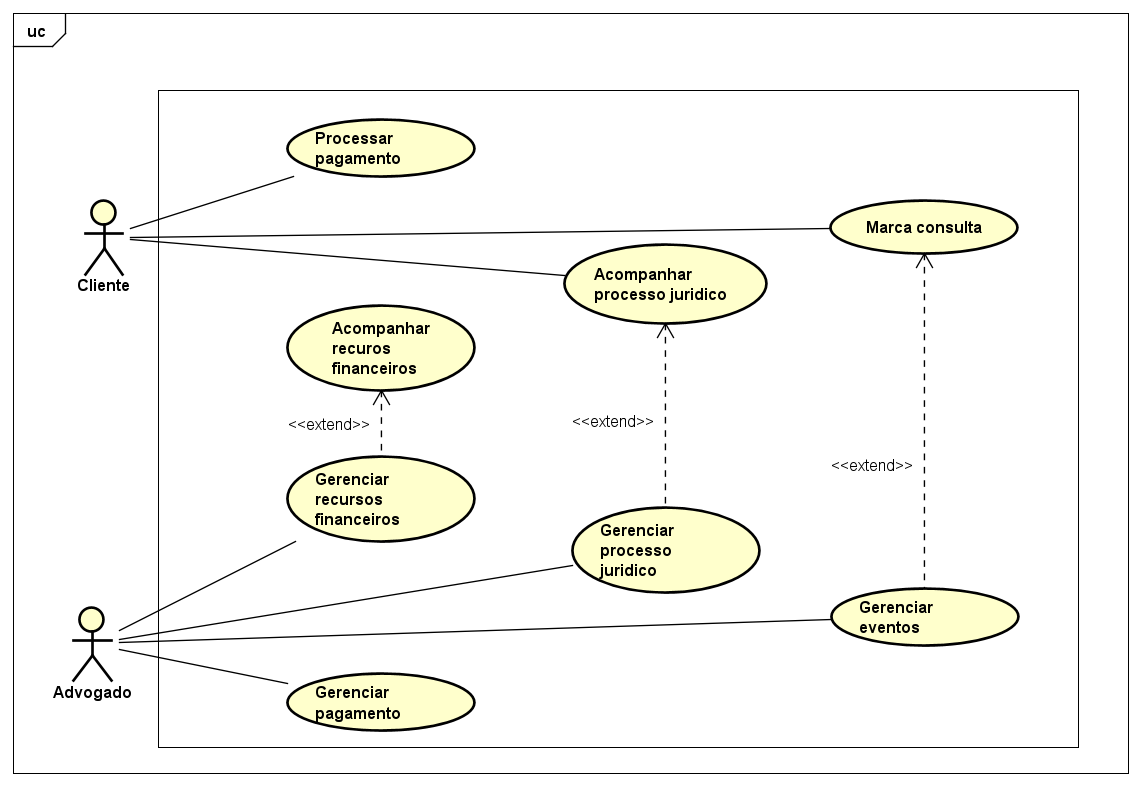
\includegraphics[width=0.8\linewidth]{imagens/Caso de uso MR Telles v5.png}
\end{figure}

Conforme detalhado na Figura 1, o ator Cliente e Advogado serão os únicos usuários ao
utilizar o sistema.
\begin{itemize}
    \item \textbf{Cliente}: Responsável por pagamentos, acompanhamento financeiro, seus processos e consultas.
    \item \textbf{Administrador (Advogado)}: Gerencia todas as funcionalidades do sistema.
\end{itemize}


\begin{enumerate}[leftmargin=*]
    \item \textbf{Processar Pagamento} (Cliente)
    \begin{itemize}
        \item Visualização de parcelas mensais
        \item Geração de QR Code PIX
        \item Confirmação manual pelo administrador
    \end{itemize}
    
    \item \textbf{Gerenciar Pagamento} (Administrador)
    \begin{itemize}
        \item Geração de PIX avulso para não cadastrados
        \item Identificação do pagador no histórico
        \item Armazenamento em lista de transações
    \end{itemize}

    \item \textbf{Acompanhar Recursos Financeiros} (Cliente)
    \begin{itemize}
        \item Visualização de parcelas pendentes
        \item Informações de valor, vencimento e status
        \item Acompanhamento de obrigações financeiras
    \end{itemize}

    \item \textbf{Gerenciar Recursos Financeiros} (Administrador)
    \begin{itemize}
        \item Cadastro de parcelas por cliente
        \item Atualização de status de pagamento
        \item Histórico financeiro
    \end{itemize}
    
    \item \textbf{Acompanhar Processo Jurídico} (Cliente)
    \begin{itemize}
        \item Consulta de andamentos processuais
        \item Visualização de histórico
        \item Detalhamento de etapas
    \end{itemize}
    
    \item \textbf{Gerenciar Processo Jurídico} (Administrador)
    \begin{itemize}
        \item Cadastro de novos processos
        \item Atualização de etapas
        \item Registro de decisões judiciais
    \end{itemize}
    
    \item \textbf{Marcar Consulta} (Cliente)
    \begin{itemize}
        \item Agendamento por calendário interativo
        \item Seleção de horários disponíveis
        \item Cancelamento de agendamentos
    \end{itemize}
    
    \item \textbf{Gerenciar Eventos} (Administrador)
    \begin{itemize}
        \item Controle completo de agenda
        \item Reagendamento de consultas
        \item Cadastro de eventos internos
    \end{itemize}
\end{enumerate}


\newpage
\section{Diagrama de Classes}\label{sec:diagrama-classes}

Na Figura \ref{fig:16}, observa-se a definição de seis classes principais para o sistema MR Telles. As classes \texttt{User}, \texttt{ControleFinanceiro}, \texttt{Processo} e \texttt{Schedule} concentram os relacionamentos centrais do sistema, compartilhando informações entre si e possibilitando a automação de funcionalidades jurídicas e financeiras.

As classes \texttt{Histórico} e \texttt{PhiTransaction} não se conectam diretamente a todas as entidades, mas são essenciais para garantir o registro de ações e a flexibilidade no controle de transações. Além disso, o diagrama representa os vínculos como associação, agregação e composição entre as classes, oferecendo suporte à rastreabilidade, gestão processual e controle de eventos.


\begin{figure}[!ht]
    \centering
    \caption{Diagrama de Classe}
    \label{fig:16}
    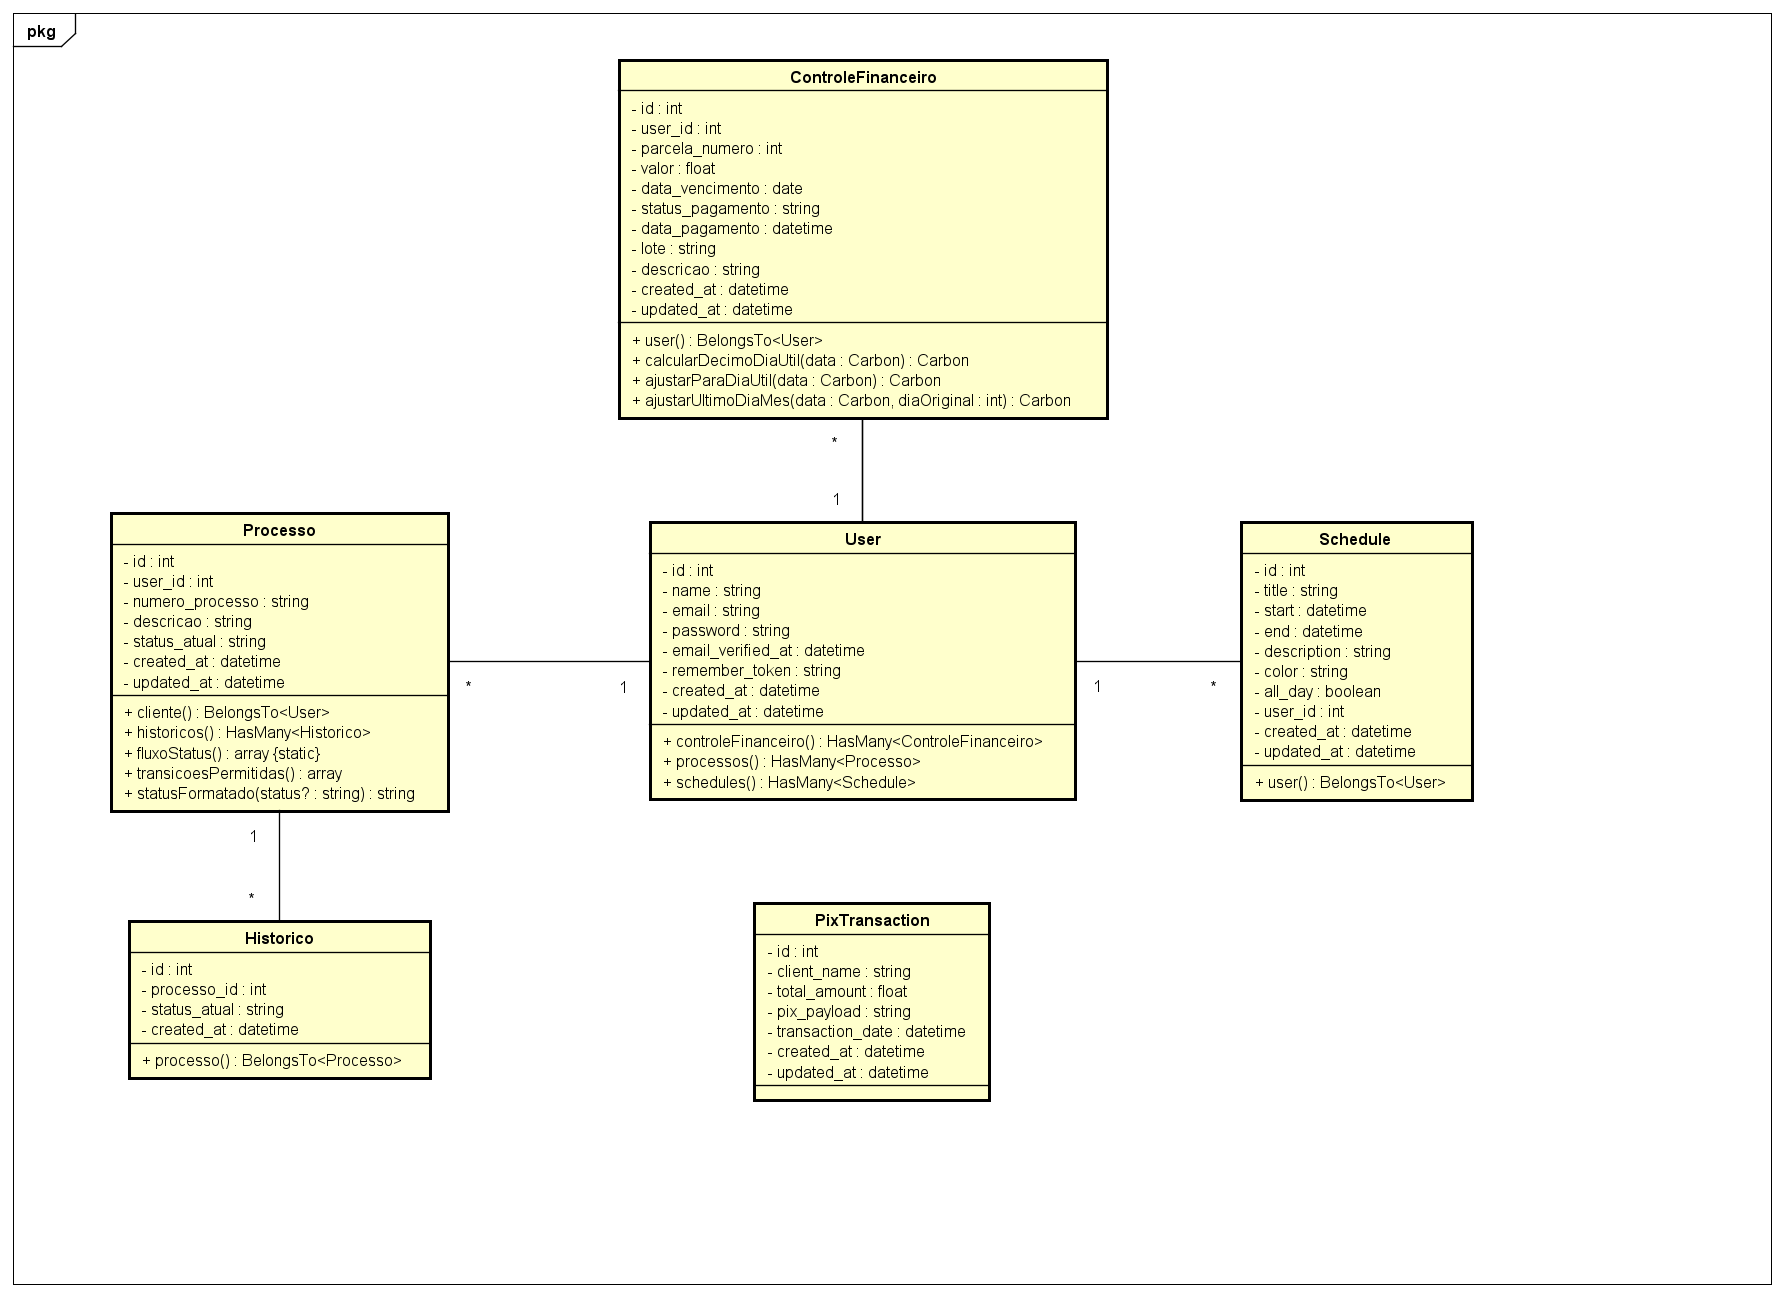
\includegraphics[width=0.8\linewidth]{imagens/uml/diagrama de classe MR Telles.png}
\end{figure}


\newpage
\section{Diagrama Entidade Relacionamento}
Na Figura \ref{fig:17}, é apresentado o diagrama entidade relacionamento (DER) é uma representação gráfica que descreve a estrutura de um banco de dados, mostrando entidades, atributos e relacionamentos. Ele é usado para modelar dados, facilitando o entendimento e o design do esquema de banco de dados. O DER do sistema MR Telles, que ilustra a estrutura do banco de dados. As principais entidades incluem users, controle financeiro, processos, historicos, schedules e pix transactions list. A entidade users está no centro da estrutura, relacionando-se diretamente com o controle financeiro, processos jurídicos e agendamento de eventos.

\begin{figure}[!ht]
    \centering
    \caption{Diagrama Entidade Relacionamento}
    \label{fig:17}
    \includegraphics[width=0.8\linewidth]{imagens/uml/Der.png}
\end{figure}

\newpage
\section{Diagrama de Implantação}
Na Figura \ref{fig:18}, o diagrama de implantação do sistema MR Telles apresenta uma arquitetura cliente-servidor convencional, onde a aplicação web é hospedada no serviço de cloud InfinityFree, executando-se sobre um sistema operacional genérico. Os usuários acessam o sistema através de navegadores web (browsers) em suas máquinas locais, que se comunicam com o servidor via protocolos TCP/IP pela internet. O armazenamento de dados é gerenciado pelo SGBD MySQL, que opera em conjunto com a aplicação web para persistência das informações.

\begin{figure}[!ht]
    \centering
    \caption{Diagrama de Implantação}
    \label{fig:18}
    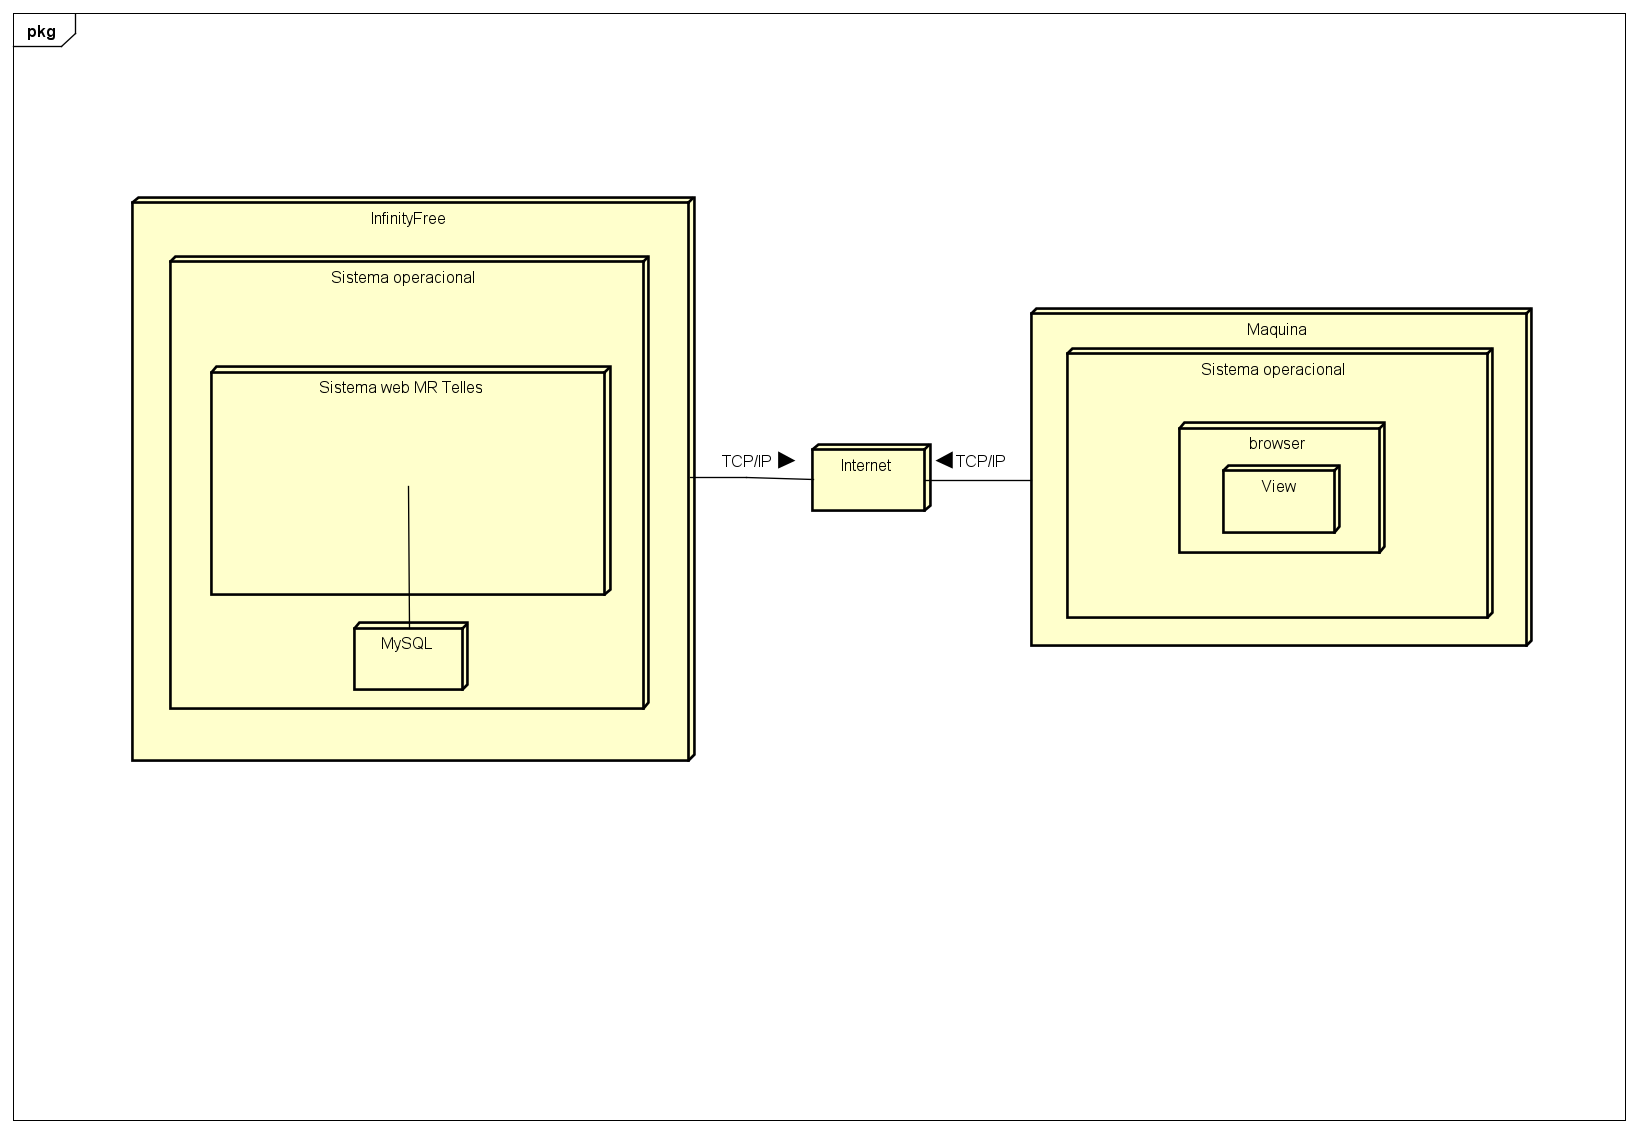
\includegraphics[width=0.8\linewidth]{imagens/uml/diagrama de implantação.png}
\end{figure}
